%%%%%%%%%%%%%%%%%%%%%%%%%%%%%%%
%This is the article LaTeX template for RSC journals
%Copyright The Royal Society of Chemistry 2010
%%%%%%%%%%%%%%%%%%%%%%%%%%%%%%%


\documentclass[8.5pt,twoside,twocolumn]{article}
\oddsidemargin -1.2cm
\evensidemargin -1.2cm
\textwidth 18cm
\headheight 1.0in
\topmargin -3.5cm
\textheight 22cm
\usepackage[super,sort&compress,comma]{natbib} 
\usepackage{mhchem}
\usepackage{times,mathptmx}
%\usepackage{times}
% feel free not to use mathptmx if it causes difficulties
\usepackage{sectsty}
\usepackage{balance} 
\usepackage{color}
\usepackage{float}
\newcommand{\e}[1]{\times10^{#1}}
\newcommand{\beq}{\begin{equation}}
\newcommand{\eeq}{\end{equation}}
\newcommand{\beqa}{\begin{eqnarray}}
\newcommand{\eeqa}{\end{eqnarray}}
\newcommand{\com}[1]{\textcolor{red}{#1}}
\newcommand{\cur}[1]{{\textit{#1}}}
\newcommand{\ben}{\begin{enumerate}}
\newcommand{\een}{\end{enumerate}}
\newcommand{\bit}{\begin{itemize}}
\newcommand{\eit}{\end{itemize}}

\usepackage{graphicx} %eps figures can be used instead
\usepackage{lastpage}
\usepackage[format=plain,justification=raggedright,singlelinecheck=false,font=small,labelfont=bf,labelsep=space]{caption} 
\usepackage{fancyhdr}
\pagestyle{fancy}

\begin{document}

\thispagestyle{plain}
\fancypagestyle{plain}{
\fancyhead[L]{
\includegraphics[height=8pt]{LH}}
\fancyhead[C]{\hspace{-1cm}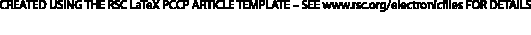
\includegraphics[height=20pt]{CH}}
\fancyhead[R]{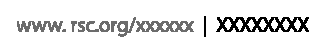
\includegraphics[height=10pt]{RH}\vspace{-0.2cm}}
\renewcommand{\headrulewidth}{1pt}}
\renewcommand{\thefootnote}{\fnsymbol{footnote}}
\renewcommand\footnoterule{\vspace*{1pt}% 
\hrule width 3.4in height 0.4pt \vspace*{5pt}} 
\setcounter{secnumdepth}{5}

\makeatletter 
\def\subsubsection{\@startsection{subsubsection}{3}{10pt}{-1.25ex plus -1ex minus -.1ex}{0ex plus 0ex}{\normalsize\bf}} 
\def\paragraph{\@startsection{paragraph}{4}{10pt}{-1.25ex plus -1ex minus -.1ex}{0ex plus 0ex}{\normalsize\textit}} 
\renewcommand\@biblabel[1]{#1}            
\renewcommand\@makefntext[1]% 
{\noindent\makebox[0pt][r]{\@thefnmark\,}#1}
\makeatother 
\renewcommand{\figurename}{\small{Fig.}~}
\sectionfont{\large}
\subsectionfont{\normalsize} 

\fancyfoot{}
\fancyfoot[LO,RE]{\vspace{-7pt}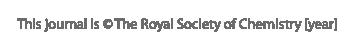
\includegraphics[height=9pt]{LF}}
\fancyfoot[CO]{\vspace{-7.2pt}\hspace{12.2cm}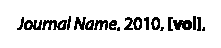
\includegraphics{RF}}
\fancyfoot[CE]{\vspace{-7.5pt}\hspace{-13.5cm}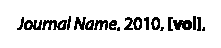
\includegraphics{RF}}
\fancyfoot[RO]{\footnotesize{\sffamily{1--\pageref{LastPage} ~\textbar  \hspace{2pt}\thepage}}}
\fancyfoot[LE]{\footnotesize{\sffamily{\thepage~\textbar\hspace{3.45cm} 1--\pageref{LastPage}}}}
\fancyhead{}
\renewcommand{\headrulewidth}{1pt} 
\renewcommand{\footrulewidth}{1pt}
\setlength{\arrayrulewidth}{1pt}
\setlength{\columnsep}{6.5mm}
\setlength\bibsep{1pt}

\twocolumn[
  \begin{@twocolumnfalse}
\noindent\LARGE{\textbf{Mesoscopic Modelling and Simulation of Soft Matter}}
\vspace{0.6cm}

\noindent\large{\textbf{Oliver Henrich \textit{$^{a}$} and Peter V. Coveney \textit{$^{b}$}}}\vspace{0.5cm}
%Please note that \ast indicates the corresponding author(s) but no footnote text is required. 


\noindent\textit{\small{\textbf{Received Xth XXXXXXXXXX 20XX, Accepted Xth XXXXXXXXX 20XX\newline
First published on the web Xth XXXXXXXXXX 200X}}}

\noindent \textbf{\small{DOI: }}
\vspace{0.6cm}
%Please do not change this text.

\noindent \normalsize{}
\vspace{0.5cm}
 \end{@twocolumnfalse}
  ]

%\footnotetext{\dag~Electronic Supplementary Information (ESI) available: [details of any supplementary information available should be included here]. See DOI: 10.1039/b000000x/}

%Please use \dag to cite the ESI in the main text of the article.
%If you article does not have ESI please remove the the \dag symbol from the title and the above footnotetext.

\footnotetext{\textit{$^{a}$~EPCC, SUPA, School of Physics and Astronomy, University of Edinburgh,\\King's Buildings, James Clerk Maxwell Building, Peter Guthrie Tait Road, Edinburgh EH9 3FD, UK\\E-mail: ohenrich@epcc.ed.ac.uk}}
\footnotetext{\textit{$^{b}$~Centre for Computational Science, University College London,\\20 Gordon Street, London WC1H 0AJ, UK}}

%additional addresses can be cited as above using the lower-case letters, c, d, e... If all authors are from the same address, no letter is required

%\footnotetext{\ddag~Additional footnotes to the title and authors can be included \emph{e.g.}\ `Present address:' or `These authors contributed equally to this work' as above using the symbols: \ddag, \textsection, and \P. Please place the appropriate symbol next to the author's name and include a \texttt{\textbackslash footnotetext} entry in the the correct place in the list.}


\section{Introduction}

Soft condensed matter \cite{Doi:2013, Terentjev:2015} is ubiquitous in our world and we 
encounter it in our everyday lives. Many complex fluids like polymer and colloidal solutions, 
liquid crystals, foams, gels, granular materials 
and biological materials belong to this category. A peculiarity that distinguishes soft matter from
 more conventional condensed matter, is that its fundamental building blocks show a 
remarkable tendency 
to self-organise into more complex structures on intermediate, mesoscopic length and time scales. 
Instances of typical time and length scale separation in soft matter are solvent mediated 
interactions of suspended colloidal particles or systems with internal degrees of freedom 
like membranes, polymer chains or vesicles. This phenomenon of self-organisation 
occurs several orders of magnitude above the molecular level, 
but on time and length scales significantly smaller than the macroscopic one.
It is a characteristic feature of soft matter, which introduces a multiscale aspect 
into the problem. This is one of the reason why describing soft condensed matter 
in a consistent way is difficult and forms a formidable challenge. 

For an understanding of the dynamical behaviour and response of soft matter it is 
essential to find coarse-grained descriptions where time and length scales can be bridged.
This is realised by representing a large number of degrees of freedom through a much 
smaller number of effective degrees of freedom whilst retaining enough of the relevant physics. 
Often nonlinear coupling mechanisms between different constituting components 
make analytical solving of the equations of motion practically impossible. 
Although flow in soft matter is usually isothermal, incompressible and is characterised
by low Reynolds numbers, hydrodynamic interactions can play an important role.
They entail long-ranged, collective interactions, but are notoriously difficult to include. 
On the other hand the rise of computing power provides the backdrop for studying soft matter 
on unprecedented scales as computer simulations have now become a third paradigm 
in science besides experiment and theory.

All these aspects together led to the development of numerous, specialised 
simulation methods for soft condensed matter, which have mostly evaded the texbook level.
The scope of this tutorial review is to introduce the most common and versatile methods,
provide an overview of their different flavours and a guide for further reading. We also like to 
round up this review with a glance at the most exciting recent applications.

\section{Mesoscopic Hydrodynamic Methods}

\subsection{Dissipative Particle Dynamics and Brownian Dynamics}

Dissipative Particle Dynamics (DPD) is a stochastic simulation method specifically designed for soft matter
and complex fluids. It was first formulated by Hoogerbrugge and Koelman 
\cite{Hoogerbrugge:1992, Koelman:1993} and later refined by Espa\~nol \cite{Espanol:1995b} and 
Groot and Warren \cite{Groot:1997}.
The basic idea is akin to coarse-grained molecular dynamics with atoms agglomerated into larger
entities or 'beads' that interact via soft forces. 

The beads are subject to conservative forces that always contain a soft-core repulsion as well as pairwise drag
or friction forces and random forces. The force ballance can be summarised as

\beq
m_i \ddot{{\mathbf{r}}}_i=\mathbf{F}_i^C+\sum_{i\neq j}\mathbf{F}_{ij}^D + \mathbf{F}_{ij}^R
\eeq

with dissipative forces between a pair of particles $i-j$ 

\beq
\mathbf{F}_{ij}^D=-\gamma\,\omega(|\mathbf{r}_{ij}|)\frac{(\mathbf{r}_{ij}\cdot\mathbf{v}_{ij})\mathbf{r}_{ij}}{|\mathbf{r}_{ij}|}
\eeq

and random forces 

\beq
\mathbf{F}_{ij}^R=\sqrt{2 k_B T \gamma\, \omega(|\mathbf{r}_{ij}|)} \frac{\mathbf{r}_{ij}}{|\mathbf{r}_{ij}|}\eta_{ij}.
\eeq

The quantity $\eta$ is a Gaussian random number with zero mean and unit variance. $\gamma$ is a friciton coefficient and
$\omega(|\mathbf{r}_{ij}|)$ a decaying weighing function with cutoff. 
Note that contrary to Brownian dynamics, where each particles requires an independent random force in DPD the 
distance-dependent friction forces for each pair of particles entail distance dependent random forces 
in order to fulfil a fluctuation-dissipation theorem.
This has been demonstrated at Gibbsian equilibrium by Espa\~nol and Warren \cite{Espanol:1995a}.

These local, pairwise interactions of DPD fulfil Newton's third law, conserve momentum and angular momentum, 
guarantee Galilean invariance and yield hydrodynamic conservation laws on larger length scales owing to the 
particle-based nature of the algorithm a coupling and a straightforward coupling between solvent and solute.
A formulation of DPD with energy conservation was given by Espa\~nol \cite{Espanol:1997}.
Together with a modified predictor-corrector algorithm for the integration \cite{Groot:1997} or a self-consistent 
 velocity-Verlet algorithm \cite{Pagonabarraga:2001} DPD permits using larger time steps than atomistic MD 
modelling.

The thermodynamic consistency was studied by Pagonabarraga and Frenkel \cite{Pagonabarraga:2001} who also
introducted of a free-energy functional.
If different species are modelled the correct compressibility and solubility of the components, 
specified by the repulsion parameters between the different species has to be provided \cite{Groot:1997}.
Otherwise there is considerable freedom in modelling the interactions.
A coarse-graining derivation of DPD from molecular dynamics has been given by 
Flekkoy and Coveney \cite{Flekkoy:1999, Flekkoy:2000}. Starting from a 
formulation of Smoothed Particle Hydrodynamics Espa\~nol and Revenga \cite{Espanol:2003} 
established the link to DPD and gave a smoothed formulation of DPD, which 
is thermodynamically consistent and allows arbitrary equations of state. 

Because pairwise interactions have to be calculated, DPD is computationally relatively expensive and  
slower than other methods like Multi-Particle Collision Dynamics or Lattice Boltzmann.
Another disadvanteage of DPD is that momentum transport is tightly coupled to particle transport and the Schmidt numbers 
are typically low. However, a scheme for arbitrarily large Schmidt numbers has been presented by Lowe \cite{Lowe:2004}.

Further details on DPD can be found in the reviews by Nielsen \cite{Nielsen:2004} and 
Moeendarbary \cite{Moeendarbary:2009, Moeendarbary:2010}.


\subsection{Stochastic Rotation Dynamics and Multi-Particle Collision Dynamics}

Multi-Particle Collision Dynamics (MPCD) was originally introduced as Stochastic Rotation Dynamics (SRD) 
by Malevenets and Kapral \cite{Malevanets:1999, Malevanets:2000}.
MPCD is just like DPD a genuinely mesoscopic simulation method that obeys hydrodynamic conservation laws 
on the macroscopic level and draws on the idea of CG, but the particle dynamics is simplified.
It consists of two separate steps: a free streaming step that mimicks the advection of non-interacting particles,
followed by a collision step, where particles are divided into cells and momentum is exchanged between the 
particles in each cell.
The concept of MPCD is similar to the Lattice Boltzmann Method (LBM), but the difference is that no discretised Boltzmann 
equation is solved and all particles are off-grid.
The method conserves mass, momentum and energy, is unconditionally stable and an H-theorem exists as 
detailed by Malevanets \cite{Malevanets:1999} and Ihle \cite{Ihle:2003}.  
Ihle and Kroll \cite{Ihle:2001} were able to restore Galileian invariance by random shifting and back-shifting
of the cell position by a fraction of the cell size before and after each collision step.

The streaming step can be written as

\beq
\mathbf{r}_{i}(t+dt)=\mathbf{r}_{i}(t)+\mathbf{v}_{i}(t)\,dt,
\eeq

where $\mathbf{r}_{i}$ and $\mathbf{v}_{i}$ are the position and velocity of particle $i$,
In three dimensions the momentum exchange happens through a rotation of the relative velocity of each particle $i$ 
with respect to the average velocity in its cell $\mathbf{v}_{i,c}=\mathbf{v}_{i}-\mathbf{u}_c$
around a randomly chosen axis $\mathbf{a}$ with random angle $\alpha$, symbolised
through the operator $\cal{R}_{\mathbf{a}, \alpha}$:

\beq
\mathbf{v}_{i}(t+dt)=\mathbf{u}_c(t)+ {\cal{R}}_{\mathbf{a}, \alpha} \, \mathbf{v}_{i,c}(t)
\eeq

A drawback of is that the stress tensor in SRD and MPCD is generally not symmetric, which
leads to a violation of angular momentum convervation, especially for mean free paths that are 
smaller than half the size of the cells. Noguchi provided a solution for this problem \cite{Noguchi:2007, Goetze:2007}
by imposing constraints on the new relative velocities of the particles.
The according update rule for the velocity with conserved angular momentum reads

\beqa
\mathbf{v}_{i}(t+dt)&=&\mathbf{u}_c(t)+ \mathbf{v}_i^R(t) - \sum_{j\in cell} \mathbf{v}_j^R(t)/ N_c \nonumber\\
&+&\frac{m}{I} \sum_{j \in cell} [\mathbf{r}_{j,c}(t)\times(\mathbf{v}_j-\mathbf{v}_j^R)]\times \mathbf{r}_{i,c}
\eeqa

with $m$ as particle mass, $I$ the moment of inertial of the particles in the cell and 
$\mathbf{r}_{i,c}=\mathbf{r}_{i}-\mathbf{R}_{c}$ as relative postition of particle $i$ with respect to centre
of mass.

In order to obtain physically meaningful results a careful mapping of simulation paramters onto 
dimensionless quantities has to be done. This step is essential as without such a mapping it
may not be possible to address a given physical problem. Padding and Louis \cite{Padding:2006} 
gave a detailed account of how this can be performed for MPCD. 
 
The particle-based algorithm simplifies the application of boundary conditions and delivers  
a straightforward coupling between solvent and solute through an extension of the collision
stage to suspended particles. This allows to easily assess the role of 
hydrodynamic interactions. 

Another advantage is the simplicity at which thermal fluctuations can be incorporated,
something that has only recently been achieved for LBM in simple \cite{Adhikari:2005} and 
complex fluids \cite{Gross:2010}. MPCD can be actually seen as SRD with thermostats. 
This establishes a close relation of MPCD to Discrete Simulation Monte-Carlo techniques with a more 
efficient multi-particle collision step (see Bird \cite{Bird:1994}) 

A comprehensive review of the MPCD method was published by Gompper et al. \cite{Gompper:2009}.



\subsection{Lattice Boltzmann Method}

Of all methods discussed in this review the Lattice Boltzmann Method (LBM) \cite{Succi:2001, Guo:2013} 
is probably the least intuitively accessible. This is because it has not evolved from an 
adaptation of molecular dynamics. LBM was originally introduced by McNamara \cite{McNamara:1988} and 
Benzi \cite{Benzi:1992} as an improvement of older Lattice Gas Cellular Automata,
which had the goal of finding solutions to the continuum Navier-Stokes equation by 
means of simplified dynamics. 

The method is rooted in statistical 
mechanics and the kinetic theory of gases and solves the Boltzmann equation
in a fully discretised fashion.
The central quantity is the probability density function
$f(\mathbf{x}, \mathbf{c}, t)$, which measures the probability of finding
a particle at position $\mathbf{x}$ at time $t$ with velocity $\mathbf{c}$.
Under the assumption of molecular chaos $f$ is a one-particle distribution function,
i.e. the velocities of all colliding particles are uncorrelated and independent of position. 
For a fluid this assumption is well justified and its dynamic state is defined
by $f$ as a solution of the Boltzmann equation. 
In the discrete analogon, the lattice Boltzmann equation (LBE), time, configuration 
and momentum space are discretised. 
The fluid consists of ficticious quasi-particles that perform a consecutive 
collision and propagation process over the discrete lattice, that can be
summarised as

\beq\label{lbe}
f_i(\mathbf{x}+\mathbf{c}_i\, dt, t+dt)=f_i(\mathbf{x}, t)+\Omega_i(\{f(\mathbf{x},t)\}).
\eeq

The velocities $\mathbf{c}_i$ form a complete set of discrete lattice vectors that
connect each site to its nearest neighbours or next-to-nearest neighbours. 
Isotropy is broken due to the discreteness of the underlying lattice,  but it can be 
restored through an appropriate choice. This leads to the popular classification 
according to Qian \cite{Qian:1992}.
The functional $\Omega$ is the collision operator that describes the effective interactions 
between the quasi-particles. In its simplest BGK-form, named after its inventors
Bhatnagar, Gross and Krook  $\Omega$ is modelled as  
the difference between $f_i$ and a local equilibrium $f_i^{eq}$ times a reciprocal 
time scale $\tau$. The time scale is related to the viscosity $\eta$ of the fluid via 
$\eta =(\tau - 1/2)\,c_s^2\,dt$ with $c_s$ as speed of sound. The lattice Boltzmann
equation reads

\beq
\Omega_i(\{f\}) = -\frac{1}{\tau}\left(f_i - f_i^{eq}\right) - g_i
\eeq

where $g_i$ is a forcing terms that accounts for the component of an 
exteral body force $\mathbf{g}$ along the lattice direction $\mathbf{c}_i$. 
Various forms have been proposed. We mention here only those according to 
He et al. \cite{He:1998} and Guo et al. \cite{Guo:2002} 


The local equilibrium distribution function $f_i^{eq}$ of an ideal Newtonian fluid is a polynomial
in the fluid velocity $\mathbf{u}$.

\beq
f_i^{eq}(\rho, \mathbf{u})=a_i\,\rho\left(1+A\,\mathbf{u}\cdot\mathbf{c}_i + B\,(\mathbf{u}\cdot\mathbf{c}_i)^2- C\,\mathbf{u}^2\right).
\eeq

The coefficients $A, B$ and $C$ are constructed so that moments of the distribution 
function and the discrete lattice velocities reproduce the local mass and momentum density
and the shear stress:

\beqa
\rho &=& \sum_i \, f_i^{eq} = \sum_i \, f_i\\
\rho \mathbf{u} &=& \sum_i \, \mathbf{c}_i f_i^{eq} = \sum_i \, \mathbf{c}_i f_i\\ 
\rho \mathbf{u} \mathbf{u} + p \mathbf{I} &=& \sum_i \, \mathbf{c}_i \mathbf{c}_i f_i^{eq}
\eeqa

Note that the last equality in the first two equations holds because density and momentum are
conserved quantities and not altered by the collision process. The last equation contains
the ideal pressure tensor $p \delta_{\alpha \beta}$. 
For a non-ideal single-component fluid the 
equilibrium distribution function is generalised to contain higher order terms. These 
are once again matched to reproduce a modified pressure tensor  
$P_{\alpha \beta}=p\delta_{\alpha \beta} + \pi_{\alpha \beta}$ that includes the 
viscous stress tensor .

The link between the abstract LBE Eq. \ref{lbe} and the macroscopic Navier-Stokes
equation is rather obscure at this level, but can be established through a multiscale
analysis in a small parameter proportional to the Knudesen number. This procedure is also
known as Chapman-Enskog expansion \cite{Succi:2001, Guo:2013}.

d'Humi\`eres et al. \cite{dHumieres:2002} generalised the collision operator to multiple relaxation times (MRT), 
offering increased stability and allow for instance different shear and bulk viscosities, a limitation of 
the single relaxation time BGK-collision operator.    
Another fundamental strand in LBM is the development of entropic LBM by Ansumali, Karlin 
and \"Ottinger \cite{Ansumali:2003}, which is not only unconditional stable, but also posseses an
H-theorem.

A consequence of the discreteness of most underlying lattices is that Galilean invariance is generally broken.
The restriction to small Mach numbers and nearly incompressible flows limits non-Galilean errors to a minimum.
It is also possible to devise schemes that mitigate this artifact \cite{Chikatamarla:2006, Dellar:2014},
but they tend to be more intricate and take away something from the simplicity of the basic idea of LBM.

Modelling complex multiphase or multi-component fluids, particularly in complex geometries, 
has been a long-standing endavour of LBM. A number of models have been proposed, which  
differ in how the physics of the interactions between the different phases and components is
incorporated. 
The Shan-Chen model \cite{Shan:1993} is a phenomenological model based on pseudo-potentials,
which model the microscopic interactions between the different phases or components directly.
Free energy models have been introduced by Swift et al. \cite{Swift:1995, Swift:1996}.
They feature a thermodynamic pressure tensor that is derived from free energy functionals. 
The basic free energy models, although thermodynamically consistent, usually violate Galilean invariance.
Quite generally all models which involve phase boundaries or interfaces suffer from spurious 
currents, which can be reduced by using higher-order isotropic schemes \cite{Connington:2012}.

In the the standard LBM algorithm hydrodynamic flow develops without thermal noise, but 
the fluctuation-dissipation theorem can be satisfied by enforcing consitency with 
fluctuating hydrodynamics. Adhikari \cite{Adhikari:2005} showed that a thermalisation of 
the additional degrees of freedom that are not directly related to hydrodynamic observables 
lead to equipartition of the fluctuating energy on all length scales. The scheme has been 
recently extended from single phase fluids \cite{Duenweg:2007} to binary mixtures \cite{Gross:2010}.

Imposing boundary conditions in LBM needs special care. Ladd and Nguyen \cite{Nguyen:2002} 
introduced the an implicit bounce-back scheme for mobile boundaries, where overall momentum is conserved but 
locally exchanged between the fluid and boundary sites. This allows high precision even 
for small solute particles when lubrication forces are included and the bounce-back condition 
is imposed on the links. Another, conceptually simpler approach is the coupling via a dissipative, 
frictional drag force between the particle and the fluid \cite{Ahlrichs:1999}. 
A much lower number of grid points required compared to the bounce-back, but the scheme is only accurate in 
hydrodynamic far-field. Singular forces on the fluid can be regularised with suitable interpolating functions.  

For further reading on LBM we refer to the books of Succi \cite{Succi:2001} and Guo \cite{Guo:2013} and the compehensive reviews of Raabe \cite{Raabe:2004}, D\"unweg and Ladd \cite{Duenweg:2009} and Aidun and Clausen \cite{Aidun:2010}.


\subsection{Smoothed Particle Hydrodynamics}

Smoothed Particle Hydrodynamics (SPH) is another particle-based, mesh free method
that draws on the idea of replacing the actual fluid with a set of particles.
It has been originally invented by Dingold, Monaghan and Lucy
with astrophysical applications in mind, but is now gaining importance for soft matter
problems.

SPH starts neither from a statistical description as LBM does, nor does it
build on a MD-type algorithm like DPD, BD or MPCD. In SPH hydrodynamic observables 
and their spatial derivatives are discretised by means of 
weight functions.

A hydrodynamic variable $A$, e.g. the density or velocity can be represented 
through an integral interpolant like  

\beq
A(\mathbf{r})=\int A(\mathbf{r'}) W(\mathbf{r}-\mathbf{r'},h ) d\mathbf{r'}
\eeq

using a kernel $W$ which is a normalised, analytical function of $\mathbf{r}-\mathbf{r'}$,
 and becomes a $\delta-$functional for $h\to0$.  

The interpolated quantity can be discretised and approximated by replacing the integral 
as sum over a finite number of SPH-particles with mass $m_b$ and density $\rho_b$.

\beq
A(\mathbf{r})\simeq A_a= \sum_b \frac{m_b\, A(\mathbf{r}_b)}{\rho_b} \;W(\mathbf{r}_a-\mathbf{r}_b, h)
\eeq

In the same spirit the first derivative of $A$ is approximated as

\beq
\mathbf{\nabla}_a A_a= \sum_b \frac{m_b\, A(\mathbf{r}_b)}{\rho_b} \;\mathbf{\nabla}_aW(\mathbf{r}_a-\mathbf{r}_b, h).
\eeq

These discrete forms can be used directly in the hydrodynamic conservation laws.
In a Lagrangian frame that moves with the fluid the total rate of 
change of mass density can be decomposed using the continuity equation:

\beq
\frac{d\rho}{dt}=\frac{\partial\rho}{\partial t} + \mathbf{v}\cdot\mathbf{\nabla}\rho =-\mathbf{\nabla}(\rho \mathbf{v})+\mathbf{v}\cdot\mathbf{\nabla}\rho.
\eeq

The discretised form of the rate of change at particle $a$ and acceleration of particle $a$ are

\beq
\frac{d\rho_a}{dt}=\sum_b m_b (\mathbf{v}_a-\mathbf{v}_b)\,\mathbf{\nabla}_a W(\mathbf{r}_a-\mathbf{r}_b,h)
\eeq

and

\beq
\frac{d\mathbf{v}_a}{dt}=-\sum_b m_b (\frac{p_a}{\rho_a^2}+\frac{p_b}{\rho_b^2} + \pi_{a b})\,\mathbf{\nabla}_a W(\mathbf{r}_a-\mathbf{r}_b,h) + \mathbf{g}_a.
\eeq	
The quantitiy $p_a$ is the scalar pressure at particle $a$ and 
related to the density $\rho_a$ via an equation of state, for 
which various forms can be assumed. $\pi_{a b}$ is the viscous 
stress tensor, for which also various forms exist that combine
relative distances and velocities between the particles. $\mathbf{g}_a$ 
is an body external force acting on particle $a$.

For a more detailed introduction we refer the reader to the two
excellent reviews by Monaghan \cite{Monaghan:2012} and Koumoutsakos \cite{Koumoutsakos:2005}.

\subsection{Brownian and Langevin Dynamics}

\section{Applications}

\bit
\item liquid crystals: Cleaver, Zannoni
\item CG-DNA: de Pablo, Ouldrige, Doye 
\item Self-Assembly, shape: Glotzer 
\item Patchy particles, Janus particles: Sciortino, Zacharelli 
\item Polymers: Kremer, Baschnagel
\item Glasses: Barrat, Berthier, Kob 
\item Active matter: Marenduzzo, Yeomans
\item Amphiphiles, interfaces, confinement: Harting, Yeomans 
\item Transition path sampling, rare events: Dellago, Frenkel, R. Allen
\item Electrokinetics: Holm, Pagonabarraga, Lobaskin
\item Melchionna
\item Kahl
\item Likos
\item Gompper, Dhont, Ripoll, Sutmann
\item Dijkstra, Sanz, Valeriani
\item Loewen
\item Frenkel, Dobnikar
\item Boek
\item Camp
\item Klapp
\item Foffi
\item H. Tanaka
\item Bresme
\item T. Schilling
\item Horbach
\item Israelachvili
\item Karlstroem
\item Cheung
\eit

\section{Conclusions and Outlook}



\footnotesize{
\bibliography{smtutrev} %your .bib file
\bibliographystyle{rsc} %the RSC's .bst file
}

\end{document}
